\chapter{2D CNN approach}
The very fist approach we tried was to develop from scratch a 2D CNN to recognize the violence in the videos, to do that we needed to extract the frame from the videos and feed it to the AI model since a 2D CNN process images.
\section{Frame extraction}
The idea initially was to do it with the help of \textit{FFmpeg}. FFmpeg is a comprehensive software suite for recording, converting, and playing audio and video, it relies on libavcodec, a library for audio/video encoding. Following there is an example of usage.
\begin{lstlisting}[language=bash, caption={FFmpeg example}, label={lst:FFmpegExample}]
#!/bin/bash
# To force the frame rate of the output file to 24 fps:
$ ffmpeg -i input.avi -r 24 output.avi

\end{lstlisting}

Following there is the code used to extract the frames from the videos. For brevity we will show only the code used to extract the frames from the "fight" directory and the path are removed.
\begin{lstlisting}[language=bash, caption={Frame extraction}, label={lst:FrameExtraction}]

    !for f in $(ls [path_to_video]); do ffmpeg -i [path_to_video]/$f -vf fps=5 [path_to_frame]/${f%.*}-%03d.png; done;
\end{lstlisting}

This command uses FFmpeg to extract frames from a video file and save them as individual images, it iterates over each file in the specified directory and applies the FFmpeg command to convert the video to frames. The frames are saved with the same name as the original video file, followed by a three-digit number to indicate the frame sequence, the frames are saved in the specified output directory.
However, this method was found to not be flexible enough, in the light of new approach to the problem like a 3D CNN, more in the next chapter, so we decided to use a different approach, we decided extract the frames at runtime and feed them to the AI model with differences depending on the model and type of dataset fed to it. However this would have been to much of a workload, especially if we executed every time, so we decided to create a sort of cache made of pickle files \textit{.pkl}, this way we would have extracted the frames only once and then we would have loaded them. The following code shows the basic idea of the frame extraction process:

\begin{lstlisting}[language=python, caption={Pickles generation}, label={lst:PicklesGeneration}]
    # Function to load a dataset of videos with corresponding labels
   function load_video_dataset(dataset_path, pkl_config, create_on_missing):
        # Initialize empty lists for training and testing data and labels
        train_data = []
        train_labels = []
        test_data = []
        test_labels = []
    
        # Generate paths for storing pickle files
        pickles_dir =  f'{ROOT_PATH}/pickles'
        pickle_name = sha256([pickle key information])
    
        # Create a list of pickle file paths
        # f'{pickles_dir}/{pickle_name}-train_data.pkl'
        # f'{pickles_dir}/{pickle_name}-train_labels.pkl'
        # f'{pickles_dir}/{pickle_name}-test_data.pkl'
        # f'{pickles_dir}/{pickle_name}-test_labels.pkl'
        try:
            # Attempt to load data and labels from pickle files
            load_data_from_pickles([pickle_file_paths...])
    
        except FileNotFoundError:
            if create_on_missing:
                # Create a list of labeled video paths from the dataset
                labelled_paths = get_labeled_video_paths(dataset_path)
    
                # Shuffle the list of labeled video paths
                # Avoid deleting always the same videos at balancing time
                shuffle(labelled_video_paths)
    
                # Load and preprocess videos,balancing
                # the number of samples for each class
                labelled_frame = balance(labelled_paths, pkl_config)
    
                # Split the data into training and testing sets
                split_data(labelled_frame, pkl_config, min_amount)
    
                # Save the data and labels as pickle files
                save_pickles([pickle_file_paths...])
    
                # Update the pickle register with 
                #the new pickle file information
                update_pickle_register(pickles_dir, pickle_name, pkl_config)
    
        except Exception as e:
            print(f"An unexpected error occurred: {e}")
    
        # Return the loaded or newly created data and labels
        return train_data, train_labels, test_data, test_labels
    

\end{lstlisting}
The main idea is to create a 4 pickle files for each configuration (train\_data, train\_label, test\_data, test\_label), the pickle files are created only if they are not present, this way we can load them at runtime and avoid the frame extraction process. In case of creation needed, the frames are shuffled and then balanced, this is done to avoid deleting always the same videos. This process allows us not only to create pickles for 2D CNN but also for 3D CNN. The \textit{pkl\_config} parameters contains a dictionary with the following information:
\begin{itemize}
	\item frame size
	\item number of frames
	\item train split
	\item fps
	\item crop
\end{itemize}
The \textit{frame size} is the size of the frame, the \textit{number of frames} is the number of frames to be extracted from the video for each \textit{burst}, the \textit{train split} is the split between training and testing, the \textit{fps} is the frame per second of the video, for example if we want to train a 2D CNN both the \textit{number of frames} and the \textit{fps} will be 1, if we want to train a 3D CNN with burst of 2 seconds we will set the \textit{number of frames} to 10 and the \textit{fps} to 5. The \textit{crop} is a boolean value that indicates if the frame should be cropped or not to remove the black bars, more on that later.

\section{Dataset cleaning}
As previously stated the dataset was very dirty, this problem would be a constant problem throughout the project, the dataset was composed of videos of different length, different resolution and different frame rate, in addition many videos contained black bars on the sides making any AI model learn from that instead of the actual features. To solve this problem we decided to crop the videos remove the black bars, this was done with the following code:

\begin{lstlisting}[language=Python, caption={Image Cropper}, label={lst:ImageCropper}]
    def crop(image, y_nonzero, x_nonzero):
    # If y_nonzero and x_nonzero are not provided, calculate them from the grayscale version of the image
    if y_nonzero is None or x_nonzero is None:
        gray_image = cv2.cvtColor(image, cv2.COLOR_BGR2GRAY)
        y_nonzero, x_nonzero = np.where(gray_image > 1)

    # Crop the image based on the calculated non-zero values
    cropped_image = image[np.min(y_nonzero):np.max(y_nonzero), np.min(x_nonzero):np.max(x_nonzero)]

    # Return the cropped image along with updated y_nonzero and x_nonzero values
    return cropped_image, y_nonzero, x_nonzero
\end{lstlisting}

However this proved to be not enough, the dataset was still very dirty, as previously said, things like writings in the videos, \textit{fake} violence frames and other problems increased the difficulty for the model to learn the correct features. Ideally we could crop the videos in a square shape starting from the center, but this would cause a too big of a loss of information, especially if we consider that the video are not centered on the violent actions. The best solution would be to have bounding boxes for each video, but alas this was not the case and to manually made it would have been too much of a workload.

\section{First model}
For the first model we decided to use a 2D CNN, the model was composed of 2 convolutional layers, 2 max pooling layers and 2 fully connected layers, the model was trained for 30 epochs with a batch size of 32, patient 15 and the restore best weight flag, the optimizer used was Adam. This parameters were found to be the best from early experimentation runs. The model was trained on the dataset with the black bars removed, the dataset was composed of 2 classes, violence and no-violence, the model was trained on 80\% of the dataset and tested on the remaining 20\%, the validation set was 30\% of the training set with a hold out methodology.  

\begin{figure}[]
    \centering
    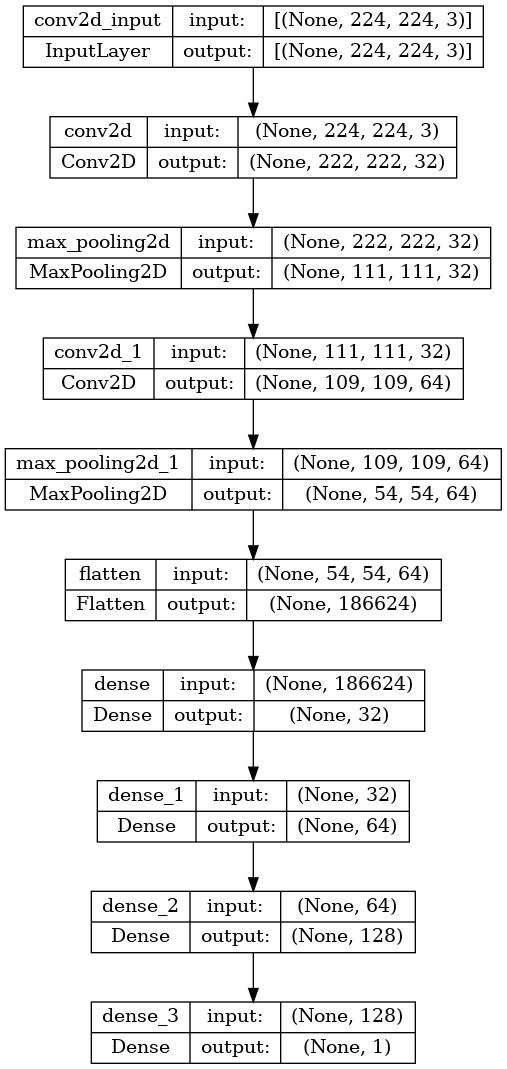
\includegraphics[width=0.8\textwidth, height=0.6\textwidth, keepaspectratio]{images/2D_3_noDrop.png}
    \caption{Initial 2D CNN model}
    \label{fig:First2DCNN}
\end{figure}

\begin{figure}[]
    \centering
    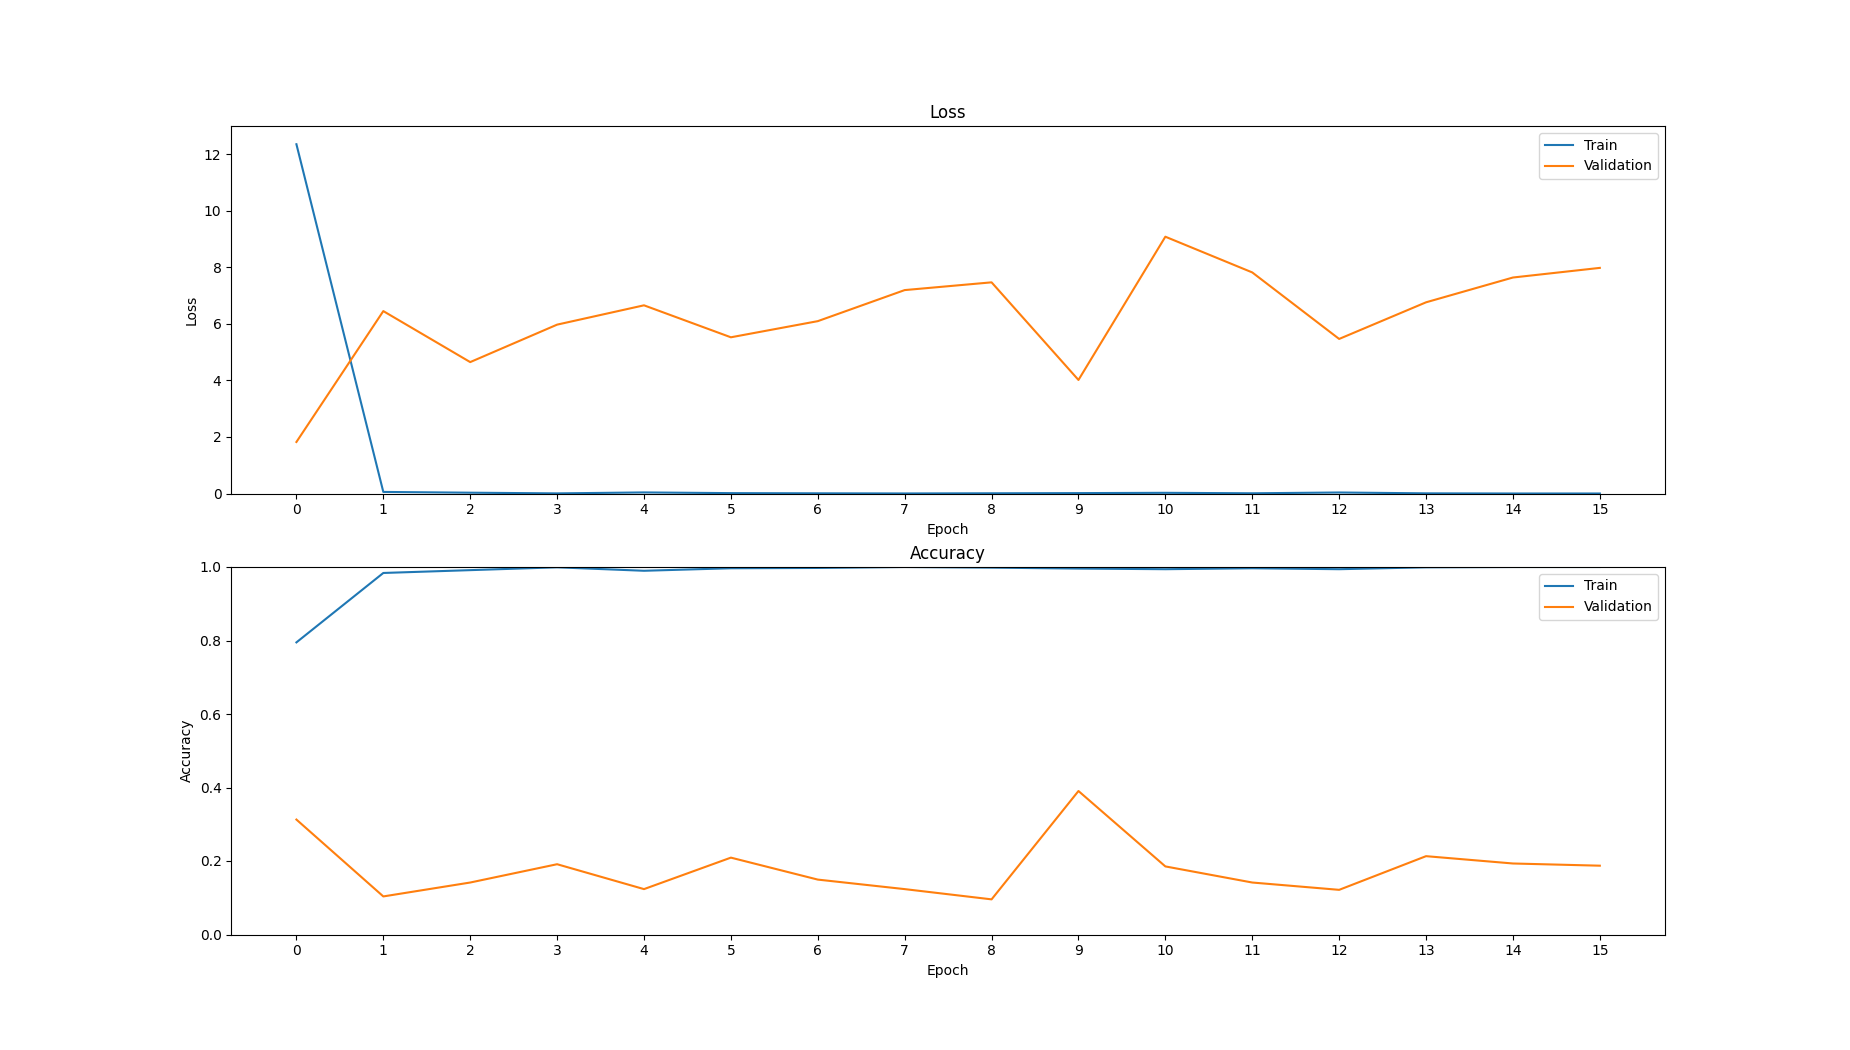
\includegraphics[width=1\textwidth]{images/731a-2D3-86ad-history.png}
    \caption{Training history of the first model}
    \label{fig:First2DCNNHistory}
\end{figure}

\begin{figure}[]
    \centering
    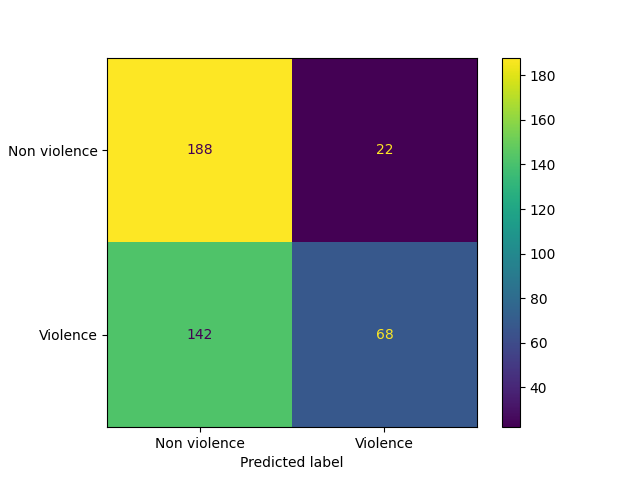
\includegraphics[width=0.8\textwidth]{images/731a-2D3-86ad-conf_matrix.png}
    \caption{Confusion matrix of the first model}
    \label{fig:First2DCNNConfusionMatrix}
\end{figure}


The first comment to be made is that the confusion matrix is heavily bias towards the \textit{Non violence} side. This is due to the fact that the dataset can be quite chaotic and the model is not able to learn the features of the videos. For example the model may learn form the Non violence part of the dataset that gatherings of people are not to be flagged as violence, however this could easily lead to false positive (Violence images classified as Non violence ones).

Another comment is to be made regarding the validation loss and accuracy which is quite unstable and unsatisfactory, this could signal overfitting and general failing in extrapolating the main features of the videos.
\pagebreak
\section{Second model}
For the second model we decided to amp the convolution layers to 3 as shown in Fig. \ref{fig:Second2DCNN}, other parameters remained unchanged this was done to see if the model would have been able to learn more features from the videos. 
We decided to use a cautious approach since the problem presented itself as a very complicated one and we did not want to aport to many changes in a single \textit{pass} to avoid a time consuming trial and error process. As can be seen in Tab. \ref{tab:2DConfront} the second model performed better than the first one by a small margin, but alas the confusion matrix is more balanced in respect to the first one, this could indicate a better generalization capability. Speaking of generalization capability, the validation loss and accuracy are still quite unstable and unsatisfactory as shown in Fig. \ref*{fig:Second2DCNNHistory}, so this must be addressed in the next models.
\begin{table}[H]
    \centering
    \resizebox{\textwidth}{!}{%
    \begin{tabular}{c|ccc|ccc|}
    \cline{2-7}
                                                & \multicolumn{3}{c|}{\textbf{FIRST MODEL}}                                                          & \multicolumn{3}{c|}{\textbf{SECOND MODEL}}                                                         \\ \cline{2-7} 
                                                & \multicolumn{1}{c|}{\textbf{PRECISION}} & \multicolumn{1}{c|}{\textbf{RECALL}} & \textbf{F1-SCORE} & \multicolumn{1}{c|}{\textbf{PRECISION}} & \multicolumn{1}{c|}{\textbf{RECALL}} & \textbf{F1-SCORE} \\ \hline
    \multicolumn{1}{|c|}{\textbf{ACCURACY}}     & \multicolumn{1}{c|}{}                   & \multicolumn{1}{c|}{}                & \textbf{0.60952}  & \multicolumn{1}{c|}{}                   & \multicolumn{1}{c|}{}                & \textbf{0.62381}  \\ \hline
    \multicolumn{1}{|c|}{\textbf{MACRO AVG}}    & \multicolumn{1}{c|}{0.66163}            & \multicolumn{1}{c|}{0.60952}         & 0.57481           & \multicolumn{1}{c|}{0.62494}            & \multicolumn{1}{c|}{0.62381}         & 0.62295           \\ \hline
    \multicolumn{1}{|c|}{\textbf{WEIGHTED AVG}} & \multicolumn{1}{c|}{0.66263}            & \multicolumn{1}{c|}{0.60952}         & 0.57481           & \multicolumn{1}{c|}{0.62494}            & \multicolumn{1}{c|}{0.62381}         & 0.62295           \\ \hline
    \end{tabular}%
    }
    \caption{Confront between the two models}
    \label{tab:2DConfront}
    \end{table}

\begin{figure}[]
    \centering
    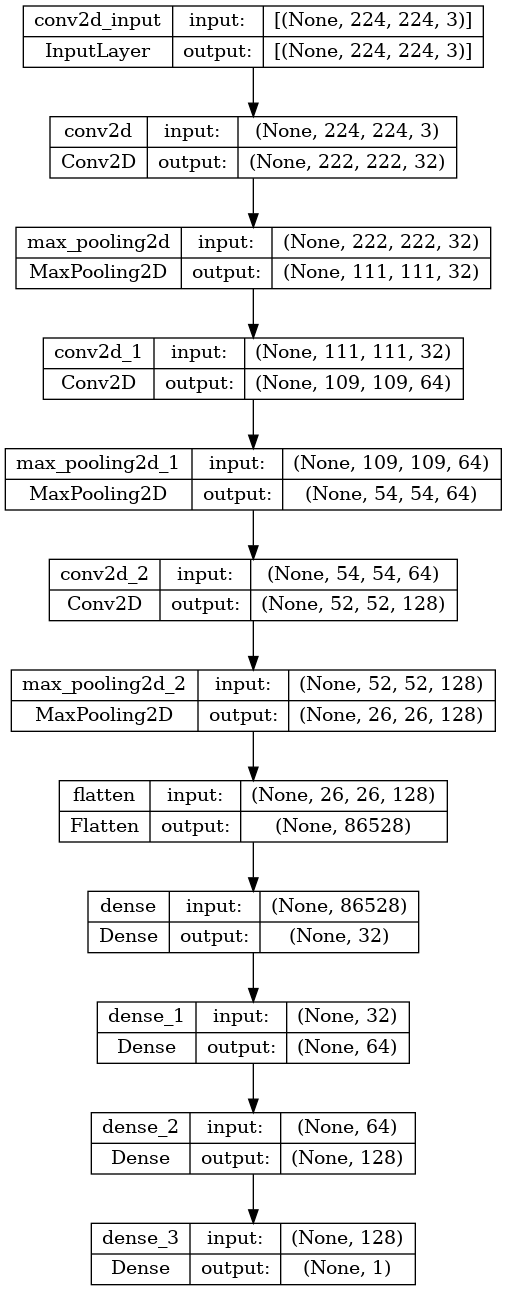
\includegraphics[width=0.8\textwidth, height=0.6\textwidth, keepaspectratio]{images/2D_35_noDrop.png}
    \caption{Second 2D CNN model}
    \label{fig:Second2DCNN}
\end{figure}


\begin{figure}[]
    \centering
    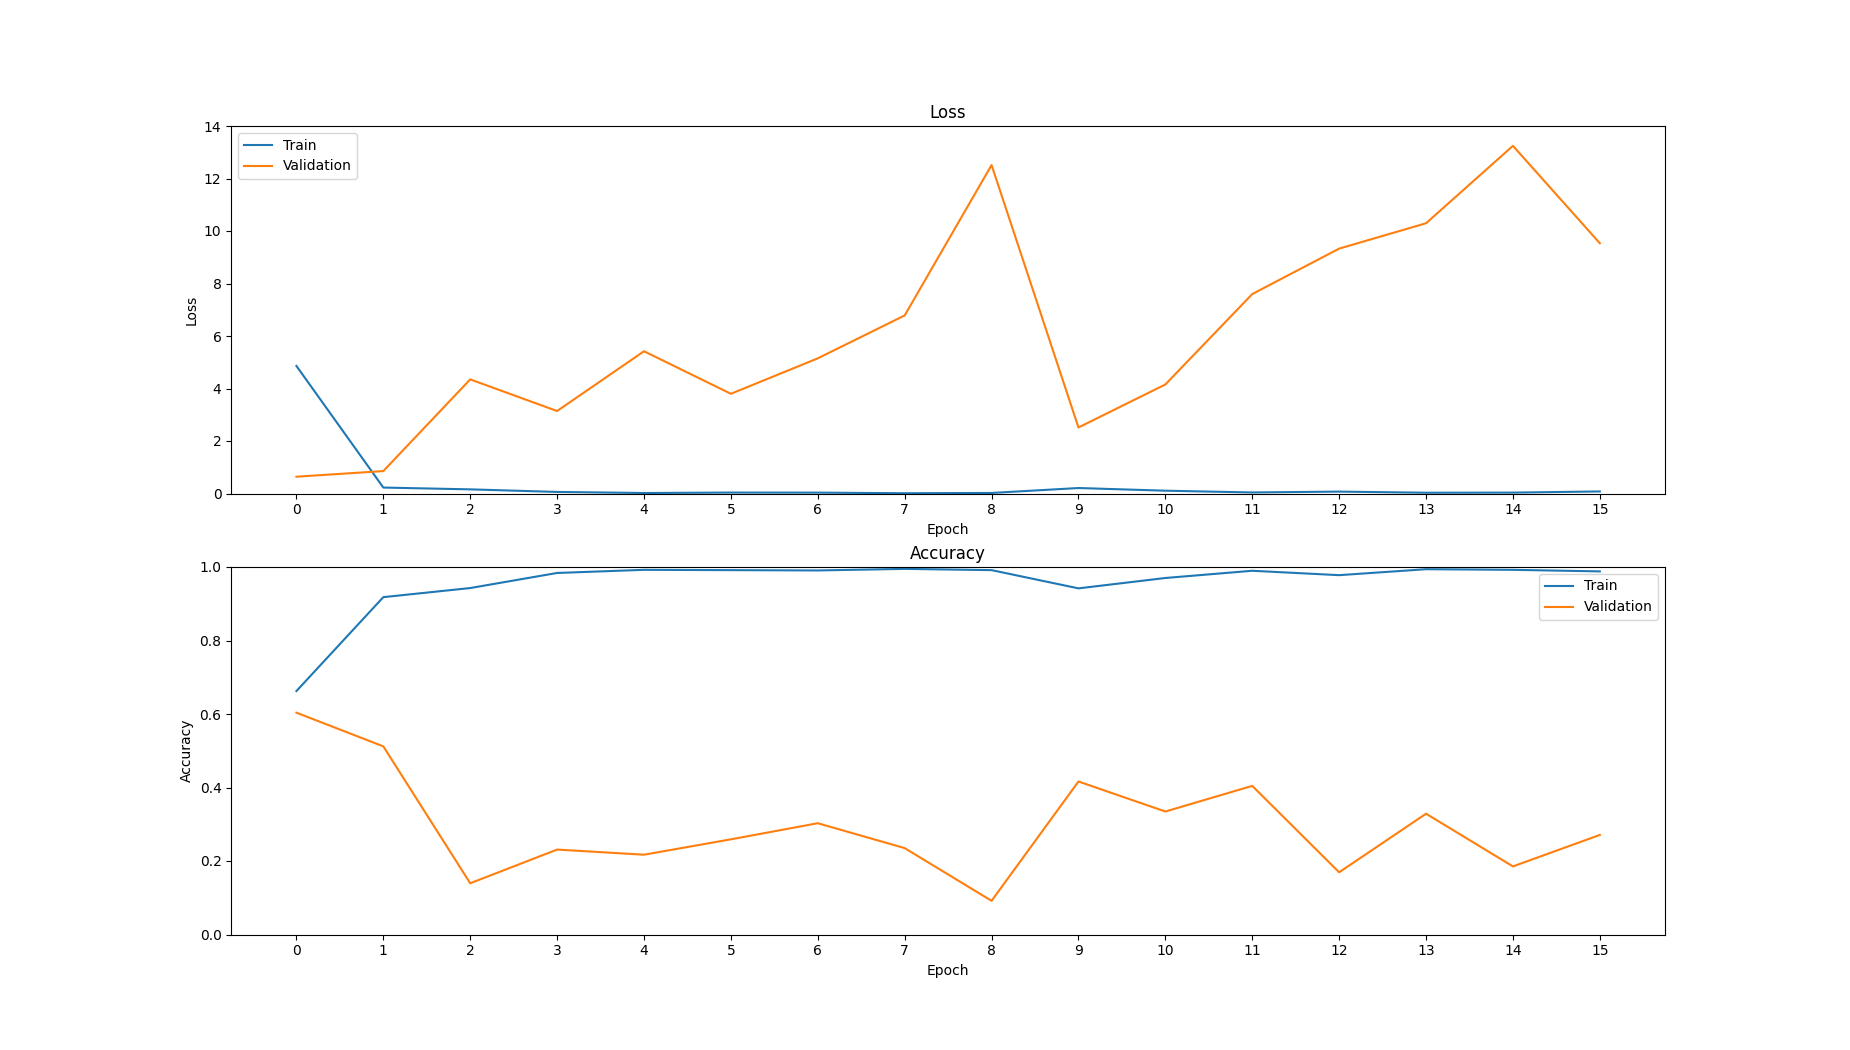
\includegraphics[width=1\textwidth]{images/731a-2D35-86ad-history.png}
    \caption{Training history of the second model}
    \label{fig:Second2DCNNHistory}
\end{figure}


\begin{figure}[]
    \centering
    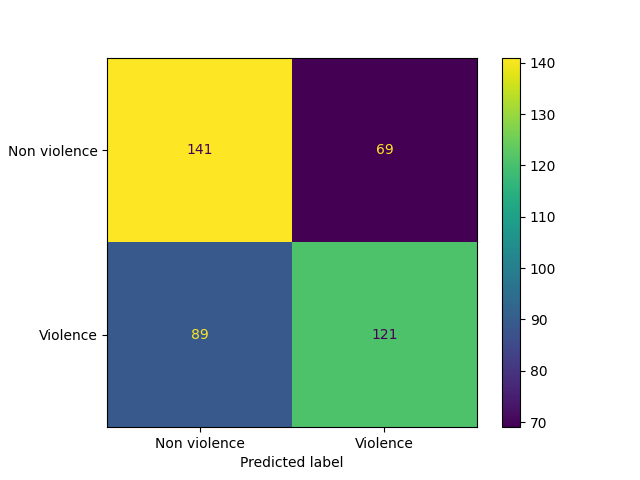
\includegraphics[width=0.8\textwidth]{images/731a-2D35-86ad-conf_matrix.png}
    \caption{Confusion matrix of the second model}
    \label{fig:Second2DCNNMatrix}
\end{figure}

\pagebreak
\section{Addressing the generalization problem}
As previously stated the generalization problem was a constant one, to addressed this we decide to add dropout layers in the model, we also decided to, according to common practice, decrease the number of dense layers. The other parameters remained unchanged. Unfortunately this did not solve the problem as shown in Fig. \ref{fig:Third2DCNNHistory} and Fig. \ref{fig:Third2DCNNMatrix}, the model is still not able to generalize well, this could be due to the fact that the dataset is too small and too dirty or the problem could be too hard to solve with a \textit{simple} 2D CNN, to achieve a better solution we would have needed a bigger dataset, but this was not available to us.
\begin{figure}[]
    \centering
    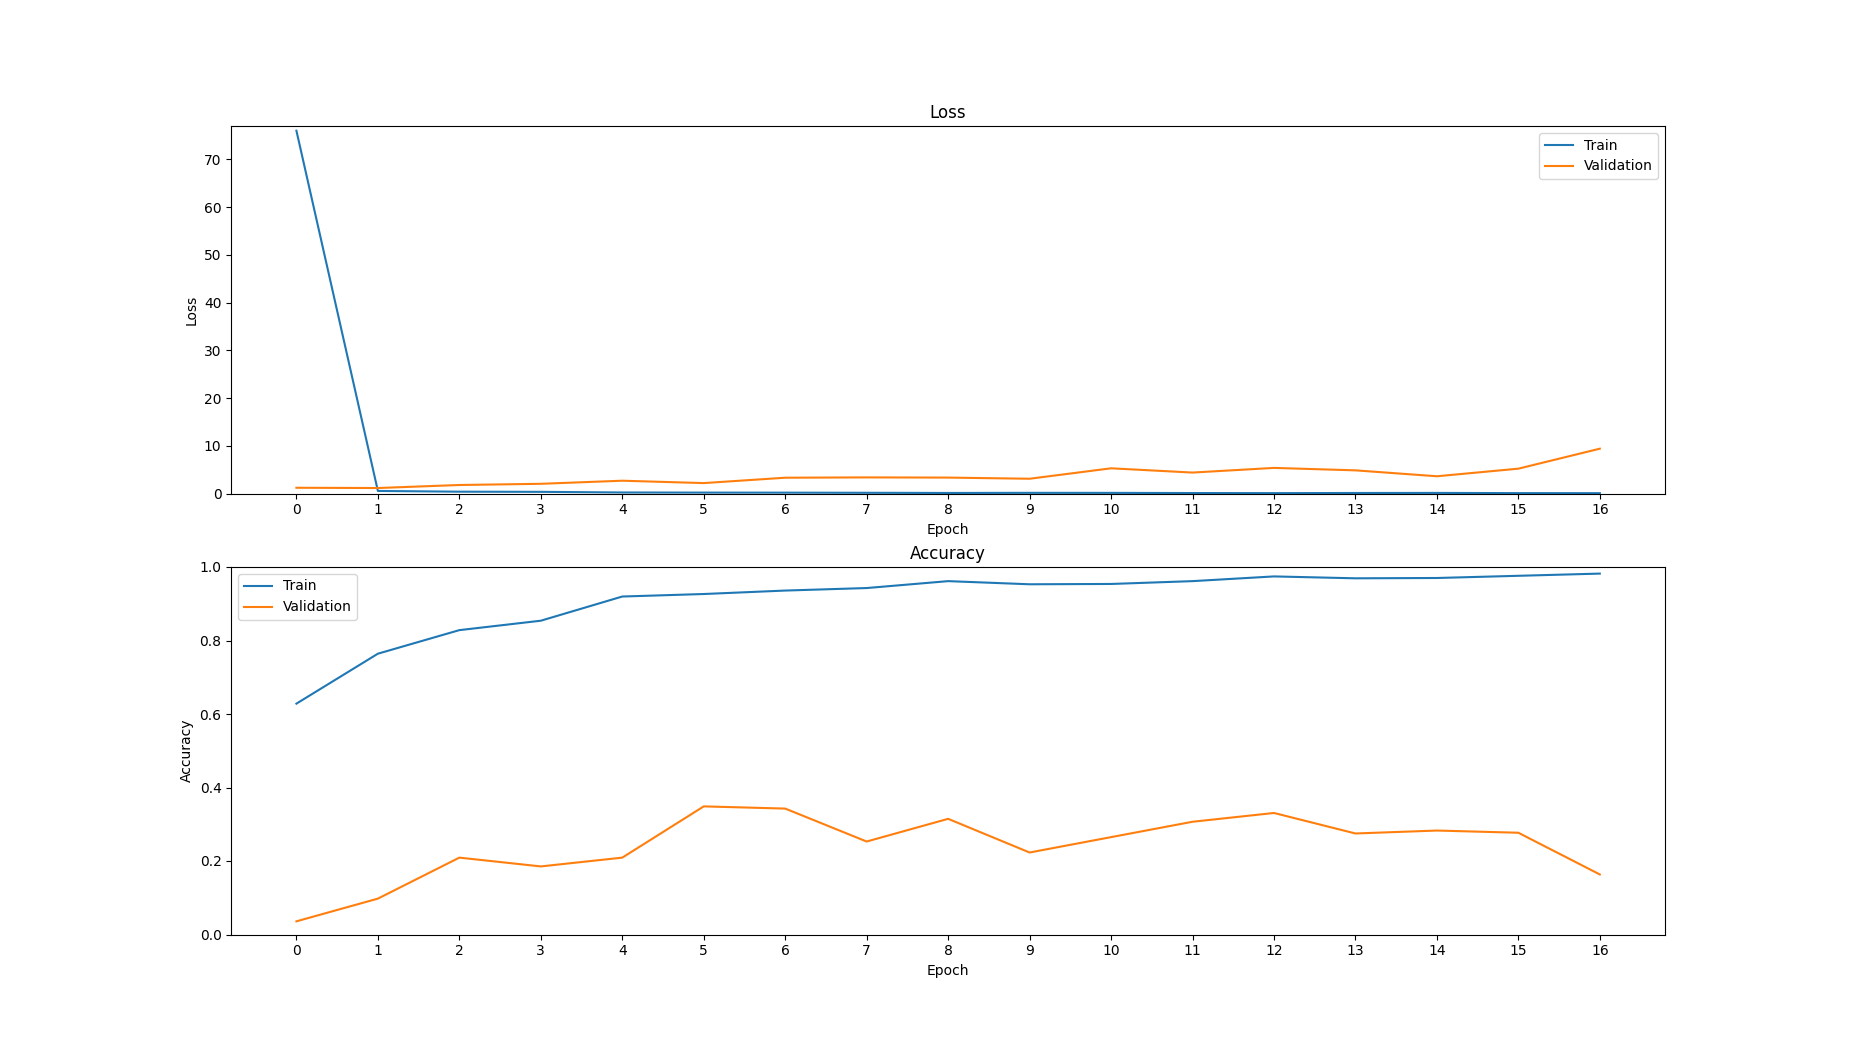
\includegraphics[width=1\textwidth]{images/731a-2DFabioFinal-86ad-history.png}
    \caption{Training history of the third model}
    \label{fig:Third2DCNNHistory}
\end{figure}
\begin{figure}[]
    \centering
    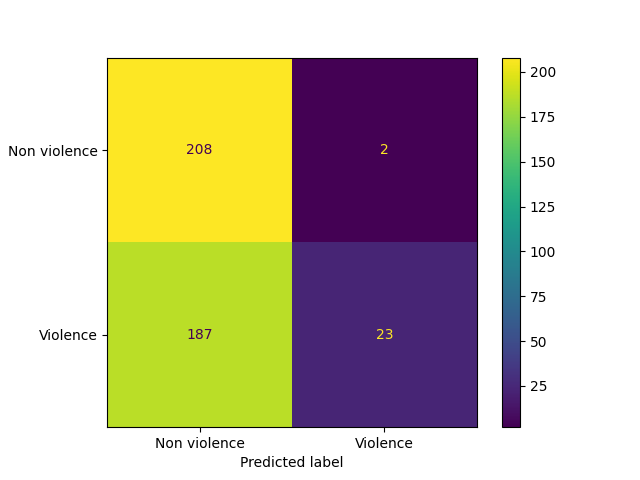
\includegraphics[width=0.8\textwidth]{images/731a-2DFabioFinal-86ad-conf_matrix.png}
    \caption{Confusion matrix of the third model}
    \label{fig:Third2DCNNMatrix}
\end{figure}
\pagebreak
\section{Fifth model}
Instead of further complicating the model we decided to simplify it to avoid the phenomenon of overfitting. The fifth model is the simplest one and has decent result, with a good recall but produces a large number of false positive as shown in  Fig. \ref{fig:FifthModelConfMatrix}. Even if this model leads to a higher accuracy and Violence recall than the previous ones, the poor Non violence recall score is too low to be considered a good model. In Tab. \ref{tab:2DCNNTable} there is a recap of the accuracy and recall of the models. The code of the fifth model is shown in the following listing: 

\begin{lstlisting}[language=python, caption={Fifth model}, label={lst:Fifth model}]
model.add(Conv2D(64, kernel_size=(3, 3), activation='relu', input_shape=input_shape))
model.add(MaxPooling2D(pool_size=(2, 2)))
model.add(Flatten())
model.add(Dense(128, activation='relu'))
model.add(Dense(64, activation='relu'))
model.add(Dense(32, activation='relu'))
model.add(Dense(1, activation='sigmoid'))
\end{lstlisting}
\begin{table}[]
    \centering
    \resizebox{\textwidth}{!}{%
    \begin{tabular}{c|c|c|c|}
    \cline{2-4}
                                                   & \textbf{Accuracy} & \textbf{Violence recall} & \textbf{Non violence recall} \\ \hline
    \multicolumn{1}{|c|}{\textbf{First Model}}     & 0,6095            & 0,3238                   & 0,8952                       \\ \hline
    \multicolumn{1}{|c|}{\textbf{Second Model}}    & 0,6238            & 0,5762                   & 0,6714                       \\ \hline
    \multicolumn{1}{|c|}{\textbf{Third Model}}     & 0,55              & 0,1095                   & 0,9905                       \\ \hline
    \multicolumn{1}{|c|}{\textbf{Final model}} & 0,7048            & 0,9095                   & 0,5                          \\ \hline
    \end{tabular}%
    }
    \caption{2D model accuracy and recall}
    \label{tab:2DCNNTable}
\end{table}

\begin{figure}[]
    \centering
    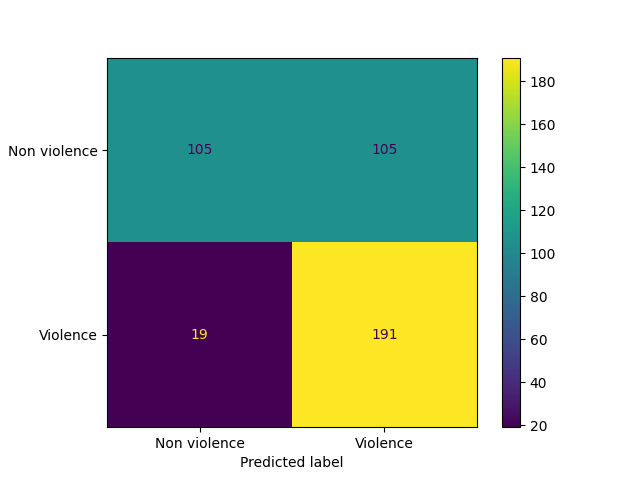
\includegraphics[width=0.8\textwidth]{images/731a-2D10_inv-86ad-conf_matrix.png}
    \caption{Fifth model}
    \label{fig:FifthModelConfMatrix}
\end{figure}

\section{Pretrained models: ResNet50}
Since the 2D \textit{from scratch} CNN approach was not working we decided to try a different method, we decided to use pretrained models. This was done to have a better understanding of the problem by comparing the results of them with the ones we presented previously. We decided to use Resnet50 as the first pretrained model. \\

ResNet50 \footnote{\url{https://arxiv.org/abs/1512.03385}} was developed by Microsoft Research in 2015, it features a deep structure with 50 layers, utilizing residual blocks that allow the network to learn residual functions to ease the optimization process.
The core innovation lies in skip connections, where the input from one layer is added to the output of another, facilitating the flow of gradients during backpropagation.
ResNet50  won the ImageNet Large Scale Visual Recognition Challenge in 2015. It includes bottleneck building blocks to improve computational efficiency by reducing the number of parameters in the intermediate layers.
\begin{figure}[]
    \centering
    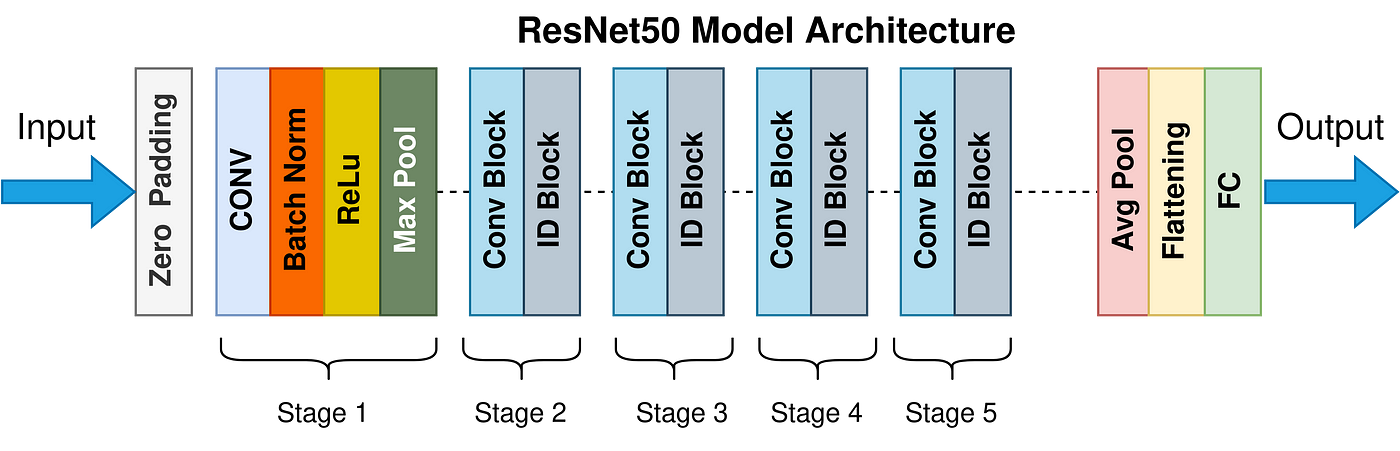
\includegraphics[width=0.8\textwidth]{images/ResNet50_architecture.png}
    \caption{ResNet50 architecture}
    \label{fig:ResNet50Arch}
\end{figure}
We used ResNet50 with the imagenet weights, and we choose to do 
\textit{fine tuning}. We started by adding our dense layers for classifications and we only train the last convolutional block.  

\begin{lstlisting}[language=python, caption={ResNet50}, label={lst:resnet50Code}]
    resnet = ResNet50(weights='imagenet', include_top=False, input_shape=input_shape)
    set_trainable = False
    for layer in resnet.layers:
        if layer.name == 'conv5_block1_1_conv':
            set_trainable = True
        if set_trainable:
            layer.trainable = True
        else:
            layer.trainable = False
    model.add(resnet)
    model.add(GlobalAveragePooling2D())
    model.add(Dense(256, activation='relu'))
    model.add(Dense(128, activation='relu'))
    model.add(Dense(1, activation='sigmoid'))
\end{lstlisting}

The model shows a promising results, with a good confusion matrix and also with a 76\% recall on violence

\begin{figure}[]
    \centering
    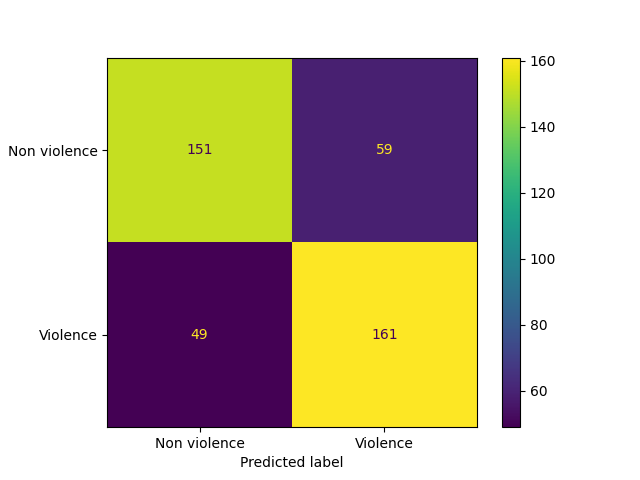
\includegraphics[width=0.8\textwidth]{images/731a-resnet2D1-86ad-conf_matrix.png}
    \caption{ResNet50 first model}
    \label{fig:ResNet2d1}
\end{figure}

We continued to improve the model adding the layers for data augmentation, however we noticed worse performances compared to the first model and signals of overfitting. 
\begin{lstlisting}[language=python, caption={ResNet50 Second Test}, label={lst:resnet50CodeSecondTest}]
    resnet = ResNet50(weights='imagenet', include_top=False, input_shape=input_shape)
    set_trainable = False
    for layer in resnet.layers:
        if layer.name == 'conv5_block1_1_conv':
            set_trainable = True
        if set_trainable:
            layer.trainable = True
        else:
            layer.trainable = False

    model.add(RandomFlip('horizontal'))
    model.add(RandomRotation(0.1))
    model.add(RandomZoom(0.2))
    model.add(resnet)
    model.add(GlobalAveragePooling2D())
    model.add(Dense(256, activation='relu'))
    model.add(Dense(128, activation='relu'))
    model.add(Dense(1, activation='sigmoid'))
\end{lstlisting}

In order to fight overfitting we introduced a dropout layer and the overall accuracy improved, and we obtained better results compared to the original model. 
\begin{figure}[h!]
    \centering
    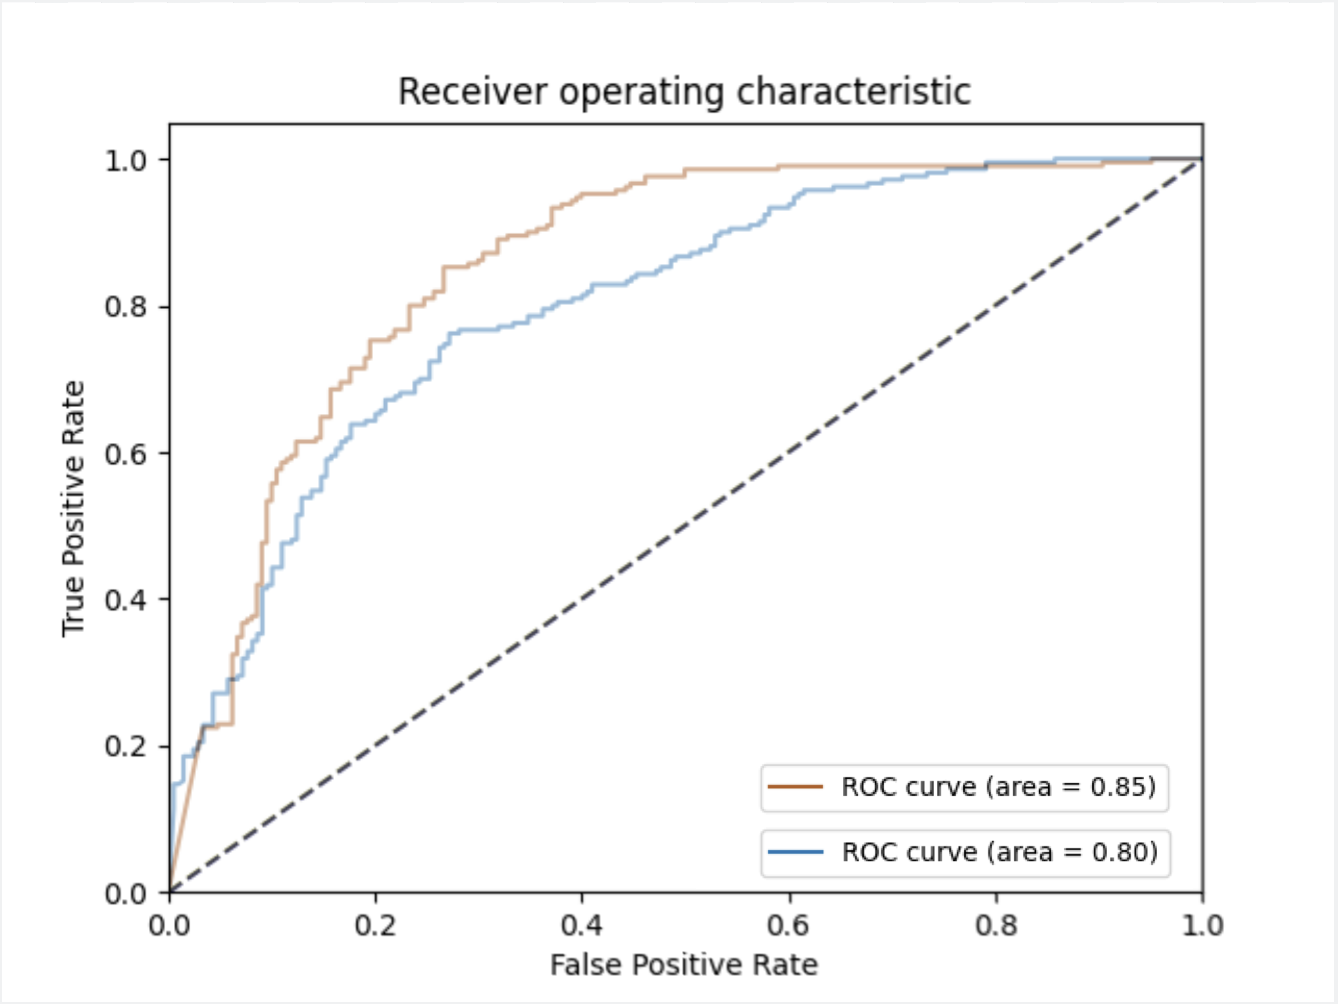
\includegraphics[width=0.8\textwidth]{images/ROCResnet.png}
    \caption{ROC of the first Resnet50 vs third Resnet50 model}
    \label{fig:ROCResnet}
\end{figure}

\begin{lstlisting}[language=python, caption={ResNet50 Third test}, label={lst:resnet50CodeThirdTest}]
    resnet = ResNet50(weights='imagenet', include_top=False, input_shape=input_shape)
    set_trainable = False
    for layer in resnet.layers:
        if layer.name == 'conv5_block1_1_conv':
            set_trainable = True
        if set_trainable:
            layer.trainable = True
        else:
            layer.trainable = False

    model.add(RandomFlip('horizontal'))
    model.add(RandomRotation(0.1))
    model.add(RandomZoom(0.2))
    model.add(resnet)
    model.add(GlobalAveragePooling2D())
    model.add(Dense(256, activation='relu'))
    model.add(Dropout(0.2))
    model.add(Dense(128, activation='relu'))
    model.add(Dense(1, activation='sigmoid'))
\end{lstlisting}


We also run a fourth test applying a small dropout also to the second dense layer but we not obtain better results compared to the previous model. We assume that our network needs the 128 neurons for a correct classification of the problem. 
\begin{lstlisting}[language=python, caption={ResNet50 Fourth test}, label={lst:resnet50CodeFourthTest}]
    resnet = ResNet50(weights='imagenet', include_top=False, input_shape=input_shape)
    set_trainable = False
    for layer in resnet.layers:
        if layer.name == 'conv5_block1_1_conv':
            set_trainable = True
        if set_trainable:
            layer.trainable = True
        else:
            layer.trainable = False

    model.add(RandomFlip('horizontal'))
    model.add(RandomRotation(0.1))
    model.add(RandomZoom(0.2))
    model.add(resnet)
    model.add(GlobalAveragePooling2D())
    model.add(Dense(256, activation='relu'))
    model.add(Dropout(0.2))
    model.add(Dense(128, activation='relu'))
    model.add(Dropout(0.1))
    model.add(Dense(1, activation='sigmoid'))
\end{lstlisting}


Following a recap of the accuracy of the models and the recall:

\begin{table}[!h]
    \centering
    \resizebox{\textwidth}{!}{%
    \begin{tabular}{c|c|c|c|}
    \cline{2-4}
                                                    & \textbf{Accuracy} & \textbf{Violence recall} & \textbf{Non Violence recall} \\ \hline
    \multicolumn{1}{|c|}{\textbf{ResNet 1st Model}} & 0,7429            & 0,7667                   & 0,7191                       \\ \hline
    \multicolumn{1}{|c|}{\textbf{ResNet 2nd Model}} & 0,6357            & 0,3619                   & 0,9095                       \\ \hline
    \multicolumn{1}{|c|}{\textbf{ResNet 3rd Model}} & 0,7643            & 0,6952                   & 0,8333                       \\ \hline
    \multicolumn{1}{|c|}{\textbf{ResNet 4th Model}} & 0,6809            & 0,6571                   & 0,7048                       \\ \hline
    \end{tabular}%
    }
    \caption{ResNet50 accuracy and recall}
    \label{tab:ResNet50}
    \end{table}

As can be seen in Tab. \ref{tab:ResNet50} the best model is the third one, this is due to the fact that the dataset is very small and the model is not able to learn from it, so the data augmentation is a must. The fourth model is not as good as the third one, because of the dropout layers which are too many and the model is not able to learn features properly. The first model is the second best and function as a base line. The second one is the worst of the collection, this is due to the fact that the data augmentation alone is not enough and also leads to overfitting of non real features as background or object in the videos.

\section{Pretrained models: EfficientNetB0}
EfficientNetB0\footnote{\url{https://arxiv.org/abs/1905.11946}} is part of the EfficientNet family, designed to achieve superior performance with fewer parameters compared to traditional models.
It introduces a compound scaling method that uniformly scales the depth, width, and resolution of the network, leading to improved efficiency across all dimensions.
The architecture includes mobile inverted bottleneck blocks and squeeze-and-excitation blocks to enhance feature extraction and model expressiveness.

EfficientNetB0 is also suitable for resource-constrained environments like mobile devices, being computationally efficient. 
\begin{figure}[h!]
    \centering
    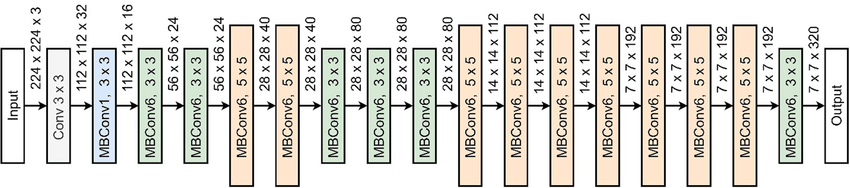
\includegraphics[width=0.8\textwidth]{images/EfficientNetB0-architecture-36.png}
    \caption{EfficientNetB0 architecture}
    \label{fig:EfficientNetB0architecture}
\end{figure}

The reason we choose EfficientNetB0 is because it can be used in IoT devices, like cameras, for a first filter on images for police operators.
Instead of going directly to fine tuning we start with a \textit{features extraction} approach.
We start from the simplest implementation as possible, with only a final dense layer with one neuron with a sigmoid activation function.
We obtained a 62\% overall accuracy, comparable to the second model of the \emph{scratch} 2D CNN but below both ResNet and the final model. In order to improve the performance of the network we add data augmentation layers and also more dense layers.
The accuracy increased from 62\% to 69\% and accordingly the violence recall (48\% compared to 38\%), however we are still far away from an acceptable level. This leads us to the conclusion that the best approach to get good results is to go to fine tuning. 
We decided to train only the two last convolutional blocks, since going at the first layers will need a huge dataset, we leave the same dense layers for classification as used in fine tuning. 
\begin{figure}[h!]
    \centering
    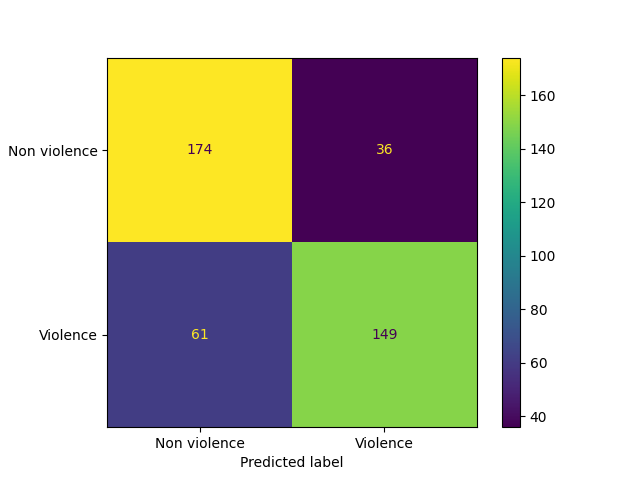
\includegraphics[width=0.8\textwidth]{images/731a-EfficientNetB0_15-5a4e-conf_matrix.png}
    \caption{EfficientNetB0: third model}
    \label{fig:EfficientNetB0_15}
\end{figure}
The results obtained are better than the ones in fine tuning, this models also obtains obtains similar results in terms of accuracy and violence recall, to the third ResNet model. 
We follow this approach unfreezing another half of the fifth convolutional blocks.
Looking at the ROC curves we cannot draw conclusions on the winner but the AUC is better and also between 0.1 and 0.8 false positive rate the fourth model performs better than the third. 

However we try to push the model to the limit adding another dense layer in order to improve the classifier performance and adding also dropout to avoid overfitting.
We obtain a good model, with a 78\% accuracy with a strong recall on violence, that we used as a second choice parameter. 
\begin{figure}[h!]
    \centering
    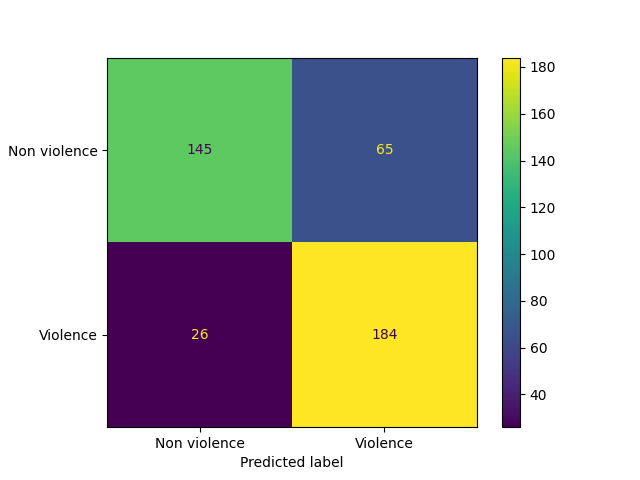
\includegraphics[width=0.8\textwidth]{images/731a-EfficientNetB0_24-b2b1-conf_matrix.png}
    \caption{EfficientNetB0: fifth model}
    \label{fig:EfficientNetB0_24}
\end{figure}

\begin{table}[]
\centering
\resizebox{\textwidth}{!}{%
\begin{tabular}{|l|l|l|l|}
\hline
                               & \textbf{Accuracy} & \textbf{Violence recall} & \textbf{Non Violence recall} \\ \hline
\textbf{Features extraction 1} & 0,6214            & 0,3857                   & 0,85714                      \\ \hline
\textbf{Features extraction 2} & 0,6928            & 0,4809                   & 0,90476                      \\ \hline
\textbf{Fine tuning 1}         & 0,7690            & 0,70952                  & 0,82857                      \\ \hline
\textbf{Fine tuning 2}         & 0,7762            & 0,7191                   & 0,8333                       \\ \hline
\textbf{Fine tuning 3}         & 0,7833            & 0,8762                   & 0,6905                       \\ \hline
\end{tabular}%
}
\caption{EfficientNetB0 accuracy and recall}
\label{tab:EfficientNetB0 }
\end{table}
\section{Reamining problems and solutions} 
The ResNet50 and EfficientNetB0 models brought some improvements to the accuracy of the model in comparison to the ones we developed, however we thought we could have done better, the main issue, as said before, is the dataset, it is too dirty and it has no action frames or bounding boxes to help the model learn the features of the videos. This leads, during the frame extract phase, to images before the violent acts or after them to be fed to the model with a violence label, this makes the model learns the wrong features. To solve this problem we could have discarded the \textit{bad} frames, but this would need to manually remove them, which would have been too much of a workload and would have been outside of the scope of the project.

    What the 2D models lack is context, if the model could evaluate more correlated frames before generating an output it would, in our minds, have been able to learn the features of the videos better, this is the main reason why the 2D models proved unsatisfactory. So we decided to try a different approach, the 3D CNN one.